% \documentclass[aspectratio=169, 11pt]{beamer}
\documentclass[aspectratio=169, 11pt, handout]{beamer}

% ── Theme ──
\usetheme{Madrid}
\usecolortheme{default}
\setbeamertemplate{navigation symbols}{}
\setbeamertemplate{footline}{%
  \leavevmode\hbox{%
    \begin{beamercolorbox}[wd=.333333\paperwidth,ht=2.5ex,dp=1ex,center]{author in head/foot}%
      \usebeamerfont{author in head/foot}\insertshortauthor
    \end{beamercolorbox}%
    \begin{beamercolorbox}[wd=.333333\paperwidth,ht=2.5ex,dp=1ex,center]{title in head/foot}%
      \usebeamerfont{title in head/foot}\insertshorttitle
    \end{beamercolorbox}%
    \begin{beamercolorbox}[wd=.333333\paperwidth,ht=2.5ex,dp=1ex,right]{date in head/foot}%
      \usebeamerfont{date in head/foot}\insertframenumber{} / \inserttotalframenumber\hspace*{2ex}
    \end{beamercolorbox}}}

% ── Packages ──
\usepackage{amsmath,amssymb}
\usepackage{booktabs}
\usepackage{xcolor}
\usepackage{colortbl}
\usepackage{graphicx}
\usepackage{tikz}
\usetikzlibrary{arrows.meta, positioning, calc}

% ── Colors ──
\definecolor{sbgreen}{HTML}{00704A}  % course accent
\definecolor{warnred}{HTML}{CC0000}
\definecolor{noteblue}{HTML}{2060A0}

% ── Commands ──
\newcommand{\E}{\mathbb{E}}
\newcommand{\Var}{\mathrm{Var}}
\newcommand{\Cov}{\mathrm{Cov}}
\newcommand{\SE}{\mathrm{SE}}
\newcommand{\Prob}{\mathrm{Pr}}
\newcommand{\indep}{\perp\!\!\!\perp}

\usepackage{soul}
\newcommand{\NUM}[2]{\sethlcolor{yellow}\hl{#1\,\textsuperscript{?}}\marginpar{\tiny #2}}
% Beamer frames are typeset inside boxes, where \marginpar raises "Not in outer par mode"
% and \marginparwidth is 4pt. Same marker; the provenance note goes to the frame footnote.
\renewcommand{\NUM}[2]{\sethlcolor{yellow}\hl{#1\,\textsuperscript{?}}\footnote[frame]{\tiny #2}}
% Compact footnote layout so several provenance notes fit under one frame.
\setbeamertemplate{footnote}{\noindent\raggedright\hspace*{0.6em}\tiny\insertfootnotemark\,\insertfootnotetext\par}
% TikZ styles used by the frames carried verbatim from old-decks/lecture05.tex (copied from its preamble).
% ── Reusable TikZ styles ──
\tikzset{
    tnode/.style={draw, rounded corners, fill=gray!10, minimum width=2.2cm, minimum height=0.65cm, font=\small, align=center},
    tgreen/.style={tnode, fill=sbgreen!15, draw=sbgreen},
    tblue/.style={tnode, fill=noteblue!12, draw=noteblue},
    tred/.style={tnode, fill=red!8, draw=warnred},
    tarrow/.style={-{Stealth}, thick}
}

% Version 2 (2026-09-28). Course spine: estimand -> identification -> estimation.
% Changes from slides.tex: m04/CHANGES-v2.md.
\newcommand{\spinestep}[1]{\textcolor{sbgreen}{\textbf{#1}}}

% ── Title ──
\title[Meeting 4]{Meeting 4: Honest Segments}
\subtitle{Applied Causal Inference for Business}
\author{Zhikun Lu}
\date{\today}

\begin{document}

% ====================================================================
\begin{frame}
\titlepage
\end{frame}

% ====================================================================
\begin{frame}{Where Does the Counterfactual Come From?}

\begin{center}
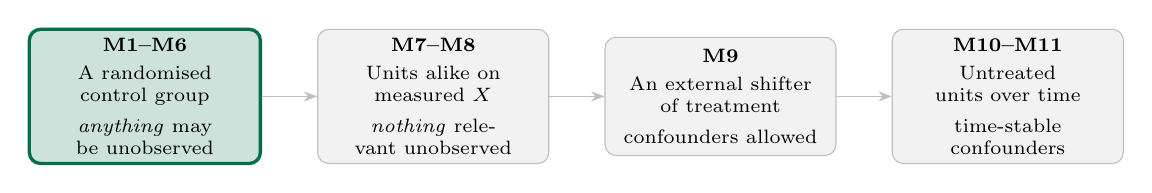
\begin{tikzpicture}[
    node distance=0.45cm and 0.7cm,
    box/.style={draw, rounded corners, minimum width=2.9cm, minimum height=1.5cm,
                font=\scriptsize, align=center, text width=2.7cm},
    active/.style={box, fill=sbgreen!20, draw=sbgreen, very thick},
    inactive/.style={box, fill=gray!10, draw=gray!50}
]
\node[active] (A) {\textbf{M1--M6}\\[2pt] A randomised control group\\[3pt] \emph{anything} may be unobserved};
\node[inactive, right=of A] (B) {\textbf{M7--M8}\\[2pt] Units alike on measured $X$\\[3pt] \emph{nothing} relevant unobserved};
\node[inactive, right=of B] (C) {\textbf{M9}\\[2pt] An external shifter of treatment\\[3pt] confounders allowed};
\node[inactive, right=of C] (D) {\textbf{M10--M11}\\[2pt] Untreated units over time\\[3pt] time-stable confounders};

\draw[-{Stealth}, gray!50] (A) -- (B);
\draw[-{Stealth}, gray!50] (B) -- (C);
\draw[-{Stealth}, gray!50] (C) -- (D);
\end{tikzpicture}
\end{center}

\bigskip

\begin{center}
\small The coin gives a clean comparison in every segment. It does not stop us from \emph{choosing}\\
the segments with the same data we use to judge them. Today: search on one half, judge on the other.
\end{center}
\end{frame}

% ====================================================================
\begin{frame}{Today's Plan}

\begin{enumerate}
    \item \spinestep{Estimand:} a segment card for store managers, the number that settles each line --- and an estimand the data will choose
    \item \spinestep{Estimation:} why outcome-based trees split on the wrong variable; splitting on the effect
    \item \textbf{H1}: committing to a partition in writing --- which fixes the estimand
    \item \spinestep{Identification and estimation,} \textbf{H2}: the fresh half, the winner's curse, what a split costs, and forests with intervals
    \item \textbf{H3}: the recommendation
\end{enumerate}

\bigskip

\textbf{Case:} Lin's coupon programme, Meeting 4 (Releases 1--5). \quad \textbf{Workshop, no AI:} honest leaves, seeds, the truth.

\bigskip

\textbf{Reading:} technical notes for Meeting 4. \quad \textbf{Due 72 hours after today:} P1.
\end{frame}

% ====================================================================
\section{The Estimand: A Segment Card}
% ====================================================================

% [RELEASE R1 — the managers' request and the rule for this analysis]
\begin{frame}{A Segment Card}

Store managers will not run a black-box score. They want a \textbf{card}: at most four segments, each marked \emph{coupon} or \emph{no coupon}.

\bigskip

Last year a consultant searched hundreds of segment definitions in a test like this one and reported a ``hidden gem'' segment with a spectacular lift. The rollout delivered a fraction of it.

\bigskip
\pause

\textbf{This time the CFO has set a rule.} Lin's Region 2 test (50/50 draw, as in Q2) is split in two:

\begin{center}
\small
\begin{tabular}{lll}
\toprule
\textbf{Step} & \textbf{Data} & \textbf{Output} \\
\midrule
\textbf{H1} discovery & half A, outcomes visible & a partition, \emph{submitted in writing} \\
\textbf{H2} estimation & half B, outcomes locked until H1 is in & one number per segment \\
\textbf{H3} recommendation & H2's numbers only & the card \\
\bottomrule
\end{tabular}
\end{center}
\end{frame}

% ====================================================================
% [RELEASE R2 — the four-cell structure of Region 2]
\begin{frame}{Region 2: Two Fields, Four Cells}

Two CRM fields: \textbf{customer type} (executive / analyst, from the job-title field) and \textbf{spending history} (high / low). Coupon randomly assigned with probability $e = 0.5$.

\begin{center}
\small
\begin{tabular}{llcccc}
\toprule
\textbf{Type} & \textbf{Spending} & \textbf{Share} & $\E[Y(1) \mid X]$ & $\E[Y(0) \mid X]$ & $\tau(x)$\\
\midrule
Executive & High & 25\% & 0.65 & 0.60 & $+0.05$ \\
Executive & Low  & 25\% & 0.35 & 0.30 & $+0.05$ \\
Analyst   & High & 25\% & 0.50 & 0.30 & $+0.20$ \\
Analyst   & Low  & 25\% & 0.20 & 0.00 & $+0.20$ \\
\bottomrule
\end{tabular}
\end{center}

\pause

\textbf{Spending history} is purely prognostic: it shifts $Y$ by $\pm 0.15$, but $\tau$ is the same across high/low.

\textbf{Customer type} is the effect modifier: $\tau(\text{analyst}) = 0.20 \neq 0.05 = \tau(\text{exec})$.

\medskip
\small Executives respond like M1's active members and analysts like the lapsed --- same effects, different purchase levels in this region. These are the truths a perfect analysis would find; the data only ever shows noisy versions.
\end{frame}

% ====================================================================
\begin{frame}{The Number That Decides It}

Each line of the card is M3's rule applied to a segment $s$: coupon iff $\tau_s > p_{1,s}/3$.

\begin{center}
\small
\begin{tabular}{llrrrr}
\toprule
\textbf{Type} & \textbf{Spending} & $\tau_s$ & $p_{1,s}$ & \textbf{Break-even} $p_{1,s}/3$ & \textbf{Net per coupon} \\
\midrule
Executive & High & 0.05 & 0.65 & 0.217 & \textcolor{warnred}{$1.50 - 6.50 = -$\textyen 5.00} \\
Executive & Low  & 0.05 & 0.35 & 0.117 & \textcolor{warnred}{$1.50 - 3.50 = -$\textyen 2.00} \\
Analyst   & High & 0.20 & 0.50 & 0.167 & \textcolor{sbgreen}{$6.00 - 5.00 = +$\textyen 1.00} \\
Analyst   & Low  & 0.20 & 0.20 & 0.067 & \textcolor{sbgreen}{$6.00 - 2.00 = +$\textyen 4.00} \\
\bottomrule
\end{tabular}
\end{center}

\pause
\bigskip

\begin{alertblock}{Every estimate today is a segment lift}
The only question is which side of \emph{its own segment's} break-even it lands on --- and whether the segment was found and judged on the same data.
\end{alertblock}

\medskip

Note the analyst--high line: a margin of $0.033$ above break-even. A segment estimate inflated or deflated by that much flips the card.
\end{frame}

% ====================================================================
\begin{frame}{An Estimand the Data Will Choose}

Until today the estimand was fixed before the data: the ATE, or $\tau(x)$ for a segment we named.

\bigskip

Today \textbf{the segments themselves come from a search}. The estimand is $\tau_\ell$ for each leaf $\ell$ of a partition that half A will suggest.

\bigskip

\begin{center}
\small
\begin{tabular}{lp{9.2cm}}
\toprule
\spinestep{Estimand} & \textbf{H1} fixes it: the partition, written down, before half B is opened \\
\spinestep{Identification} & half B's own coin, inside each committed leaf --- exactly M1's argument, on a subpopulation \\
\spinestep{Estimation} & difference in means and its SE, leaf by leaf, on half B only \\
\bottomrule
\end{tabular}
\end{center}

\bigskip

If the same data both choose the estimand and estimate it, step 1 has leaked into step 3. That is the whole of today's problem.
\end{frame}

% ====================================================================
\section{Estimation: Why Outcome Trees Split on the Wrong Thing}
% ====================================================================

% Warm-up link: the depth-one regression tree.
% [CARRIED VERBATIM from old-decks/lecture05.tex:146]
\begin{frame}{Review: How a Decision Tree Works}
 
A decision tree partitions the covariate space into leaves and predicts $\hat{Y}_\ell = \bar{Y}_\ell$ in each leaf.
 
\bigskip
 
\textbf{Splitting criterion:} choose the split that maximizes the between-group variance:
\[
\Delta_{\text{CART}}(\text{split}) = \frac{n_L}{n_P}(\bar{Y}_L - \bar{Y}_P)^2 + \frac{n_R}{n_P}(\bar{Y}_R - \bar{Y}_P)^2
\]
 
The split that creates the biggest gap in $\bar{Y}$ wins.
 
\pause
\bigskip
 
\textbf{Regularization} (minimum leaf size, maximum depth, pruning) limits the number of splits.
 
Each split must explain enough outcome variance to justify the added complexity. Variables with small outcome gaps are pruned first.
 
\end{frame}

% [CARRIED VERBATIM from old-decks/lecture05.tex:169]
\begin{frame}{The Outcome Variance Hierarchy}
 
Pool treated and control. Rank candidate splits by outcome gap:
 
\bigskip
 
\begin{center}
\begin{tabular}{lccc}
\toprule
\textbf{Candidate split} & \textbf{Gap in $\bar{Y}$} & \textbf{Gap in $\tau$} & \textbf{Rank by $\bar{Y}$} \\
\midrule
Spending history & $|0.5125 - 0.2125| = \mathbf{0.30}$ & $|0.125 - 0.125| = 0$ & 1st \\
Customer type & $|0.475 - 0.25| = 0.225$ & $|0.05 - 0.20| = \mathbf{0.15}$ & 2nd \\
Coupon $D$ & $|0.425 - 0.30| = 0.125$ & --- & 3rd \\
\bottomrule
\end{tabular}
\end{center}
 
\pause
\bigskip
 
The prognostic variable dominates. The effect modifier comes second. The treatment itself comes last.
 
Under regularization, the coupon effect (0.125) will be pruned before spending (0.30) and type (0.225).
 
\end{frame}

% [CARRIED VERBATIM from old-decks/lecture05.tex:197]
\begin{frame}{S-Learner under Strong Regularization}
 
The S-Learner fits $\hat{\mu}(X, D)$ jointly. With strong regularization, max depth = 1. The coupon $D$ competes for splits against spending and type.
 
\bigskip
 
\begin{center}
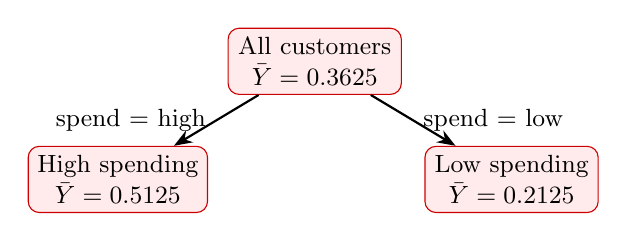
\begin{tikzpicture}
\node[tred] (root) at (0, 2.2) {All customers\\ $\bar{Y} = 0.3625$};
\node[tred] (l) at (-2.5, 0.7) {High spending\\ $\bar{Y} = 0.5125$};
\node[tred] (r) at (2.5, 0.7) {Low spending\\ $\bar{Y} = 0.2125$};
\draw[tarrow] (root) -- (l) node[midway, left, font=\small]{spend = high};
\draw[tarrow] (root) -- (r) node[midway, right, font=\small]{spend = low};
\end{tikzpicture}
\end{center}
 
\bigskip

Spending wins the first split (gap 0.30).
 
\medskip

\pause 

Coupon $D$ never enters. $\hat{\tau}(x) = \hat{\mu}(x, 1) - \hat{\mu}(x, 0) = 0$ for everyone.
 
\end{frame}

% [CARRIED VERBATIM from old-decks/lecture05.tex:228]
\begin{frame}{S-Learner under Moderate Regularization}
 
Allow two splits. After spending, the next largest gap is customer type (0.225), which still beats coupon (0.125).
 
\bigskip
 
\begin{center}
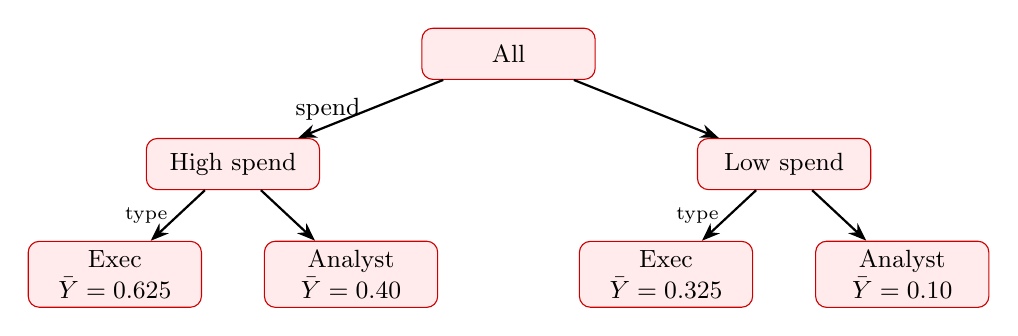
\begin{tikzpicture}[level distance=1.4cm, sibling distance=2.8cm]
\node[tred] (root) at (0, 2.8) {All};
\node[tred] (l) at (-3.5, 1.4) {High spend};
\node[tred] (r) at (3.5, 1.4) {Low spend};
\node[tred] (ll) at (-5.0, 0) {Exec\\$\bar{Y}=0.625$};
\node[tred] (lr) at (-2.0, 0) {Analyst\\$\bar{Y}=0.40$};
\node[tred] (rl) at (2.0, 0) {Exec\\$\bar{Y}=0.325$};
\node[tred] (rr) at (5.0, 0) {Analyst\\$\bar{Y}=0.10$};
\draw[tarrow] (root) -- (l) node[midway, left, font=\small]{spend};
\draw[tarrow] (root) -- (r) node[midway, right, font=\small]{};
\draw[tarrow] (l) -- (ll) node[midway, left, font=\scriptsize]{type};
\draw[tarrow] (l) -- (lr) node[midway, right, font=\scriptsize]{};
\draw[tarrow] (r) -- (rl) node[midway, left, font=\scriptsize]{type};
\draw[tarrow] (r) -- (rr) node[midway, right, font=\scriptsize]{};
\end{tikzpicture}
\end{center}
 
\pause
\medskip
 
Coupon \emph{still} never enters. Still $\hat{\tau}(x) = 0$ for everyone.
 
The S-Learner needs \textbf{three} levels of depth (spending $\to$ type $\to$ coupon) to detect any treatment effect at all.
 
\end{frame}

% [CARRIED VERBATIM from old-decks/lecture05.tex:262]
\begin{frame}{T-Learner under Regularization}
 
The T-Learner fits separate models $\hat{\mu}_1(x)$ and $\hat{\mu}_0(x)$, then subtracts.
 
\bigskip
 
\begin{center}
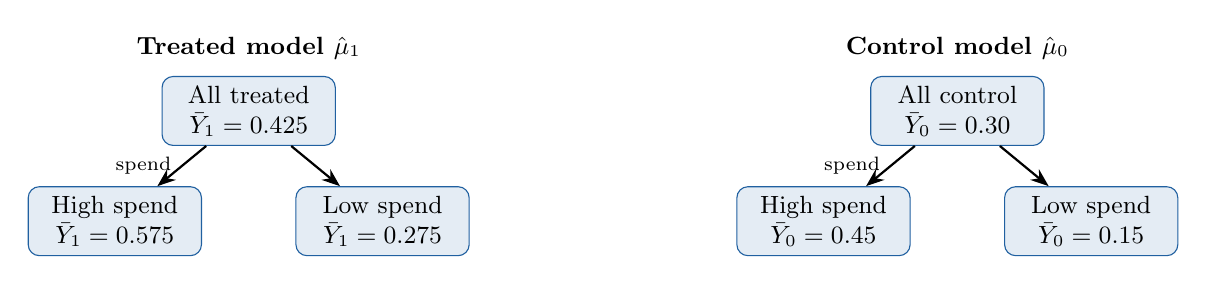
\begin{tikzpicture}
% Treated
\node[font=\small\bfseries] at (-4.5, 2.8) {Treated model $\hat{\mu}_1$};
\node[tblue] (t1) at (-4.5, 2.0) {All treated\\ $\bar{Y}_1 = 0.425$};
\node[tblue] (t1l) at (-6.2, 0.6) {High spend\\$\bar{Y}_1 = 0.575$};
\node[tblue] (t1r) at (-2.8, 0.6) {Low spend\\$\bar{Y}_1 = 0.275$};
\draw[tarrow] (t1) -- (t1l) node[midway, left, font=\scriptsize]{spend};
\draw[tarrow] (t1) -- (t1r);
 
% Control
\node[font=\small\bfseries] at (4.5, 2.8) {Control model $\hat{\mu}_0$};
\node[tblue] (t0) at (4.5, 2.0) {All control\\ $\bar{Y}_0 = 0.30$};
\node[tblue] (t0l) at (2.8, 0.6) {High spend\\$\bar{Y}_0 = 0.45$};
\node[tblue] (t0r) at (6.2, 0.6) {Low spend\\$\bar{Y}_0 = 0.15$};
\draw[tarrow] (t0) -- (t0l) node[midway, left, font=\scriptsize]{spend};
\draw[tarrow] (t0) -- (t0r);
\end{tikzpicture}
\end{center}
 
\pause
\bigskip
 
Treated arm: spending (gap 0.30) beats type (0.15). Control arm: spending and type \emph{tie} at 0.30 --- this tree breaks the tie on spending. Subtract:
\[
\hat{\tau}(\text{high}) = 0.575 - 0.45 = 0.125, \qquad \hat{\tau}(\text{low}) = 0.275 - 0.15 = 0.125
\]
 
\textcolor{warnred}{Constant $\hat{\tau}$ everywhere.} Heterogeneity by customer type completely missed.
 
\end{frame}

% [CARRIED VERBATIM from old-decks/lecture05.tex:301]
\begin{frame}{Why Prognostic Splits Waste Capacity}
 
The T-Learner's spending split explains a 0.30 gap in each arm.

\bigskip
 
But this gap \emph{cancels} in the subtraction $\hat{\mu}_1 - \hat{\mu}_0$:
\[
0.575 - 0.45 = 0.125 \quad = \quad 0.275 - 0.15 = 0.125
\]
 
\pause
\bigskip
 
The split used all of the model's capacity on a variable that is irrelevant for treatment effects.
 
\bigskip
 
Meanwhile, customer type drives a 0.15 gap in $\tau$ (analyst: 0.20 vs.\ exec: 0.05) but only a 0.15 gap in $Y$ within the treated arm. Under regularization, it loses to spending.
 
\pause
\bigskip
 
\begin{alertblock}{Core Problem}
Both the S-Learner and T-Learner select splits based on \emph{outcome} variation. Variables that predict $Y$ but not $\tau$ consume model capacity and crowd out the variables that matter for targeting.
\end{alertblock}
 
\end{frame}

% [CARRIED VERBATIM from old-decks/lecture05.tex:331]
\begin{frame}{Effect Modifiers vs.\ Prognostic Variables}
 
\textbf{Effect modifier:} $X_j$ such that $\tau(x)$ varies with $X_j$.
\begin{itemize}
    \item Customer type: $\tau(\text{analyst}) = 0.20 \neq 0.05 = \tau(\text{exec})$
\end{itemize}
 
\bigskip
 
\textbf{Prognostic variable:} $X_j$ that predicts $\E[Y \mid X]$ but not $\tau$.
\begin{itemize}
    \item Spending history: shifts $Y$ by $\pm 0.15$, zero gap in $\tau$
\end{itemize}
 
\pause
\bigskip
 
\begin{center}
\begin{tabular}{lcc}
\toprule
& \textbf{Effect modifier} & \textbf{Prognostic only} \\
\midrule
Useful for targeting? & \textcolor{sbgreen}{Yes} & \textcolor{warnred}{No} \\
Dominates regularized S-Learner? & \textcolor{warnred}{No} & \textcolor{warnred}{Yes} \\
Dominates regularized T-Learner? & \textcolor{warnred}{No} & \textcolor{warnred}{Yes} \\
Dominates Causal Tree? & \textcolor{sbgreen}{Yes} & \textcolor{sbgreen}{No} \\
\bottomrule
\end{tabular}
\end{center}
 
\end{frame}

% ====================================================================
\section{Estimation: Splitting on the Effect}
% ====================================================================

% [CARRIED VERBATIM from old-decks/lecture05.tex:369]
\begin{frame}{Step 1: The Causal Tree Splitting Criterion}
 
Replace CART's outcome gap with a \emph{treatment effect} gap:
 
\bigskip
 
\begin{block}{Causal Tree Criterion}
At each candidate split of parent $P$ into children $L$ and $R$:
\[
\Delta(\text{split}) = \frac{n_L}{n_P}\bigl(\hat{\tau}_L - \hat{\tau}_P\bigr)^2 + \frac{n_R}{n_P}\bigl(\hat{\tau}_R - \hat{\tau}_P\bigr)^2
\]
where $\hat{\tau}_\ell = \bar{Y}_{1,\ell} - \bar{Y}_{0,\ell}$ is the diff-in-means in leaf $\ell$.
\end{block}
 
\pause
\bigskip
 
A split on a purely prognostic variable produces $\hat{\tau}_L \approx \hat{\tau}_R \approx \hat{\tau}_P$, so $\Delta \approx 0$.
 
The criterion is \emph{blind} to outcome variation that does not translate into treatment effect variation.
 
\end{frame}

% ====================================================================
\begin{frame}{Causal Tree: The First Split in Region 2}

Evaluate candidate splits at the root, with the population cell effects:

\begin{center}
\begin{tabular}{lcl}
\toprule
\textbf{Candidate split} & $\Delta$ & \textbf{Decision} \\
\midrule
Spending history & $0.5(0.125 - 0.125)^2 + 0.5(0.125 - 0.125)^2 = 0$ & \textcolor{warnred}{$\Delta = 0$} \\
Customer type    & $0.5(0.05 - 0.125)^2 + 0.5(0.20 - 0.125)^2 = 0.0056$ & \textcolor{sbgreen}{Split here!} \\
\bottomrule
\end{tabular}
\end{center}

\pause
\bigskip

\begin{center}
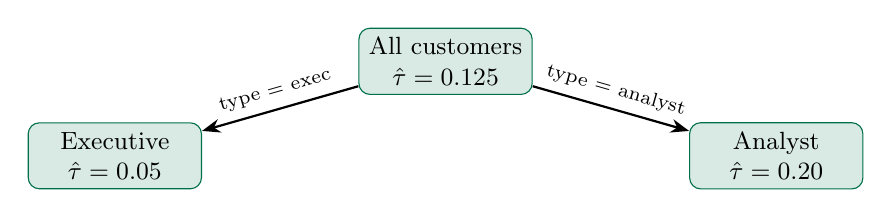
\begin{tikzpicture}
\node[tgreen] (root) at (0, 1.6) {All customers\\ $\hat{\tau} = 0.125$};
\node[tgreen] (l) at (-4.2, 0.4) {Executive\\ $\hat{\tau} = 0.05$};
\node[tgreen] (r) at (4.2, 0.4) {Analyst\\ $\hat{\tau} = 0.20$};
\draw[tarrow] (root) -- (l) node[midway, above, sloped, font=\scriptsize]{type = exec};
\draw[tarrow] (root) -- (r) node[midway, above, sloped, font=\scriptsize]{type = analyst};
\end{tikzpicture}
\end{center}

\pause

\textbf{On a sample, nothing is exactly zero.} Every candidate split shows \emph{some} $\Delta$ from noise, and the tree keeps whichever noise looks biggest. With 14 fields and a dozen cut points each, it will find something: the problem H1 and H2 are built around.
\end{frame}

% [CARRIED VERBATIM from old-decks/lecture05.tex:430]
\begin{frame}{Side-by-Side: Three Methods Compared}
 
\begin{center}
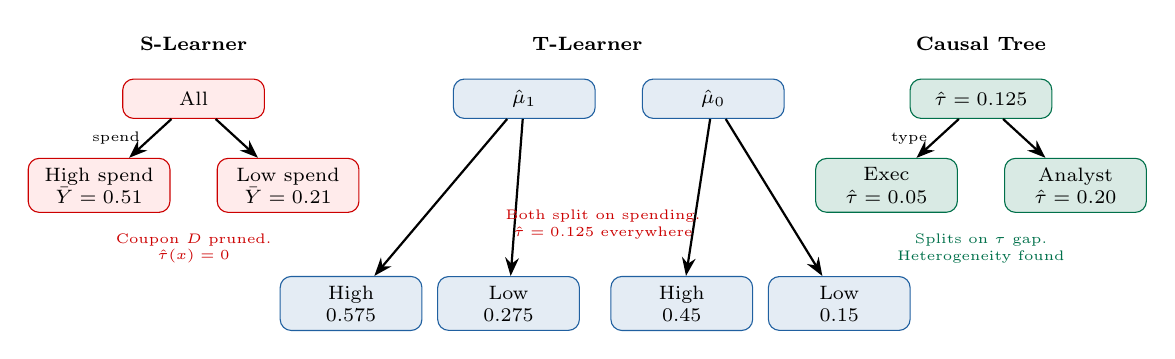
\begin{tikzpicture}[
    snode/.style={draw, rounded corners, minimum width=1.8cm, minimum height=0.5cm, font=\scriptsize, align=center},
    sg/.style={snode, fill=sbgreen!15, draw=sbgreen},
    sb/.style={snode, fill=noteblue!12, draw=noteblue},
    sr/.style={snode, fill=red!8, draw=warnred},
    sarrow/.style={-{Stealth}, thick, font=\tiny}
]
 
% S-Learner
\node[font=\scriptsize\bfseries] at (-5.0, 2.8) {S-Learner};
\node[sr] (s-root) at (-5.0, 2.1) {All};
\node[sr] (s-l) at (-6.2, 1.0) {High spend\\ $\bar{Y}=0.51$};
\node[sr] (s-r) at (-3.8, 1.0) {Low spend\\ $\bar{Y}=0.21$};
\draw[sarrow] (s-root) -- (s-l) node[midway, left]{spend};
\draw[sarrow] (s-root) -- (s-r);
\node[font=\tiny, text=warnred, align=center] at (-5.0, 0.2) {Coupon $D$ pruned.\\$\hat{\tau}(x) = 0$};
 
% T-Learner
\node[font=\scriptsize\bfseries] at (0.0, 2.8) {T-Learner};
\node[sb] (t1) at (-0.8, 2.1) {$\hat{\mu}_1$};
\node[sb] (t1l) at (-3.0, -0.5) {High\\0.575};
\node[sb] (t1r) at (-1.0, -0.5) {Low\\0.275};
\draw[sarrow] (t1) -- (t1l);
\draw[sarrow] (t1) -- (t1r);
\node[sb] (t0) at (1.6, 2.1) {$\hat{\mu}_0$};
\node[sb] (t0l) at (1.2, -0.5) {High\\0.45};
\node[sb] (t0r) at (3.2, -0.5) {Low\\0.15};
\draw[sarrow] (t0) -- (t0l);
\draw[sarrow] (t0) -- (t0r);
\node[font=\tiny, text=warnred, align=center] at (0.2, 0.5) {Both split on spending.\\$\hat{\tau}=0.125$ everywhere};
 
% Causal Tree
\node[font=\scriptsize\bfseries] at (5.0, 2.8) {Causal Tree};
\node[sg] (ct-root) at (5.0, 2.1) {$\hat{\tau} = 0.125$};
\node[sg] (ct-l) at (3.8, 1.0) {Exec\\$\hat{\tau}=0.05$};
\node[sg] (ct-r) at (6.2, 1.0) {Analyst\\$\hat{\tau}=0.20$};
\draw[sarrow] (ct-root) -- (ct-l) node[midway, left]{type};
\draw[sarrow] (ct-root) -- (ct-r);
\node[font=\tiny, text=sbgreen, align=center] at (5.0, 0.2) {Splits on $\tau$ gap.\\Heterogeneity found};
 
\end{tikzpicture}
\end{center}
 
\bigskip
 
All three use trees. Only the causal tree's splitting criterion targets treatment effect heterogeneity.
 
\end{frame}

% ====================================================================
% [RELEASE R3 — discovery half A only. Half B outcomes stay locked.]
\begin{frame}{H1: Search, Then Commit}

On half A, Lin's causal tree (all 14 fields, depth 2) returns four leaves:

\begin{center}
\small
\begin{tabular}{lrrl}
\toprule
\textbf{Leaf} & \textbf{Half-A lift} & \textbf{Break-even}$^{\dagger}$ & \textbf{Card, if we believed half A} \\
\midrule
Analyst, low spend & \NUM{0.23}{sim region2 v1: half-A leaf diff-in-means, analyst-low} & 0.067 & coupon \\
Analyst, high spend & \NUM{0.21}{sim region2 v1: half-A lift, analyst-high} & 0.167 & coupon \\
Executive, app user & \NUM{0.19}{sim region2 v1: half-A lift, exec-app (app use is not a true modifier)} & 0.167 & \textcolor{warnred}{coupon} \\
Executive, no app & \NUM{0.01}{sim region2 v1: half-A lift, exec-no-app} & 0.167 & no coupon \\
\bottomrule
\end{tabular}
\end{center}

\vspace{-0.4em}
\scriptsize $^{\dagger}$From the four-cell table; executives average $p_1 = 0.50$. \quad Where did ``app user'' come from? Nothing in M1--M3 said app use modifies the effect.

\pause
\small
\begin{alertblock}{In pairs, in writing, now}
The partition (four leaf definitions) and the card you would print. Half B's outcomes are released only after every pair has submitted.
\end{alertblock}
\vspace{0.6em}
\end{frame}

% ====================================================================
\section{H2: Identification and Estimation on the Fresh Half}
% ====================================================================

% [RELEASE R4 — half B outcomes, for the committed partition only]
\begin{frame}{H2: The Same Leaves, Estimated on Half B}

The same four leaves, each estimated on members the tree never saw:

\begin{center}
\small
\begin{tabular}{lrrrl}
\toprule
\textbf{Leaf} & \textbf{Half-B lift} & \textbf{SE} & \textbf{Break-even} & \textbf{Card} \\
\midrule
Analyst, low spend & \NUM{0.20}{sim region2 v1: half-B leaf diff-in-means, analyst-low} & \NUM{0.03}{sim v1: half-B SE, analyst-low} & 0.067 & \textcolor{sbgreen}{coupon} \\
Analyst, high spend & \NUM{0.18}{sim v1: half-B lift, analyst-high} & \NUM{0.04}{sim v1: half-B SE, analyst-high} & 0.167 & undecided \\
Executive, app user & \NUM{0.04}{sim v1: half-B lift, exec-app} & \NUM{0.05}{sim v1: half-B SE, exec-app} & 0.167 & \textcolor{warnred}{no coupon} \\
Executive, no app & \NUM{0.06}{sim v1: half-B lift, exec-no-app} & \NUM{0.03}{sim v1: half-B SE, exec-no-app} & 0.167 & no coupon \\
\bottomrule
\end{tabular}
\end{center}

\pause

\small Every leaf the search \emph{liked} came back lower; the one it liked for no reason collapsed: \textbf{executive app users are off the card}. Analyst--high now straddles its break-even.
\vspace{0.8em}
\end{frame}

% ====================================================================
% ====================================================================
\begin{frame}{Two Noisy Splits}

A discovery sample with an overall lift of $0.10$. Two candidate splits into equal halves:

\begin{center}
\begin{tabular}{lrrr}
\toprule
\textbf{Split} & \textbf{Left lift} & \textbf{Right lift} & $\Delta = 0.5(\hat\tau_L - 0.10)^2 + 0.5(\hat\tau_R - 0.10)^2$ \\
\midrule
A & 0.02 & 0.18 & $0.0064$ \\
B & 0.09 & 0.11 & $0.0001$ \\
\bottomrule
\end{tabular}
\end{center}

\bigskip

A wins. Suppose, in truth, \emph{neither} split separates anything: all four leaves have lift $0.10$. On fresh data split A gives $(0.08, 0.12)$.

\bigskip

\begin{center}
\Large the gap: $0.16 \;\longrightarrow\; 0.04$
\end{center}

\bigskip

A was chosen \emph{for} having the largest gap, and the largest gap is partly noise. Do not report the 0.16 as evidence.
\end{frame}

\begin{frame}{Why Honesty Matters: The Winner's Curse}

The splitting criterion searches over many candidate splits and picks the one with the largest $\hat{\tau}_L - \hat{\tau}_R$. The winner is selected partly on signal, partly on noise.

\pause
\medskip

\textbf{By hand.} 20 candidate segments, every one with true lift $0.125$, each estimated with SE $0.04$. The expected \emph{largest} of 20 standard normals is $1.87$, so the best-looking segment shows, on average,
\[
0.125 + 1.87 \times 0.04 = \textcolor{warnred}{0.20}
\]
--- a segment that ``beats'' the analyst--high break-even, found in data where nothing differs.

\pause
\medskip

\begin{columns}
\column{0.48\textwidth}
\textbf{Reported on half A:}\\
Leaf effects inflated toward the noise that selected them. SEs too small; intervals undercover.

\column{0.48\textwidth}
\textbf{Reported on half B:}\\
Noise in B is independent of the choice made on A. Leaf estimates are unbiased given the partition.
\end{columns}

\medskip
\textbf{The cost:} each half does its job with half the data. Honesty trades variance for a number you can act on.
\end{frame}

% ====================================================================
\begin{frame}{What Honesty Costs --- and What a Split Costs}

\textbf{Honesty's price.} Estimating on half the data doubles a leaf's variance: $s^2 \to 2s^2$.

\textbf{The alternative's price.} Reporting the winner on the data that chose it adds a squared bias of $(s \cdot \E[\max_{j \leq k} Z_j])^2$: already larger than $s^2$ at $k = 4$ candidates ($1.03^2$). A tree search compares hundreds.

\bigskip

\textbf{A split must earn its cost.} A leaf with 100 members per arm, buying at $0.30$ with the coupon and $0.10$ without:
\[
\SE = \sqrt{\tfrac{0.21}{100} + \tfrac{0.09}{100}} = 0.055 .
\]
Split it into two halves with the \emph{same} rates: each SE becomes $\sqrt{\tfrac{0.21}{50} + \tfrac{0.09}{50}} = 0.077$. Same effects, more noise, nothing gained.

\bigskip

\small This is why trees need minimum leaf sizes, and why a split is kept only if it changes the \emph{decision}.
\end{frame}

% ====================================================================
\begin{frame}{What Must Be True for H2}

From the CFO's rule and Lin's log:

\bigskip

\begin{center}
\small
\begin{tabular}{p{6.2cm}p{6.8cm}}
\toprule
\textbf{The case says} & \textbf{Which buys} \\
\midrule
``Members were split into halves by a random draw on member ID, before anyone looked.'' & A and B come from the same population: B can judge A's segments. \\[0.4em]
``Half B's outcomes were held by the CFO's office until every partition was submitted.'' & \textbf{Honesty:} the partition cannot depend on B's noise. \\[0.4em]
``Each half kept its own 50/50 coupon draw.'' & Within every leaf of B, the difference in means is unbiased for the leaf's CATE. \\
\bottomrule
\end{tabular}
\end{center}

\bigskip
\pause

The middle sentence is the one that matters and the one most often broken --- by an analyst who ``just checks'' B while tuning the tree. After that, B is discovery data too.

\medskip
\small Forests use the same idea inside every tree, and add a second ingredient: each tree sees a \emph{subsample} drawn without replacement.
\end{frame}

% [CARRIED VERBATIM from old-decks/lecture05.tex:617]
\begin{frame}{Honesty vs.\ Cross-Validation}
 
Both hold out data to address overfitting. They solve different problems.
 
\bigskip
 
\begin{center}
\begin{tabular}{p{4.0cm}p{4.0cm}p{4.0cm}}
\toprule
& \textbf{Cross-Validation} & \textbf{Honesty} \\
\midrule
\textbf{Goal} & Select model complexity & Enable valid inference on $\hat{\tau}(x)$ \\[0.4em]
\textbf{What is held out?} & Prediction error on new folds & Structural decisions (splits) \\[0.4em]
\textbf{Fixes adaptive bias?} & \textcolor{warnred}{No} & \textcolor{sbgreen}{Yes} \\[0.4em]
\textbf{Used in} & Any ML model & Causal trees and forests \\
\bottomrule
\end{tabular}
\end{center}
 
\bigskip
 
A cross-validated T-Learner selects the best outcome model, but its CATE estimates are still computed on data that influenced the model structure. Its intervals for $\hat\tau(x)$ are not valid when computed on the data that chose the model; honest or cross-fitted estimation is needed.
 
\end{frame}

% ====================================================================
\section{Estimation: From One Tree to a Forest}
% ====================================================================

% [CARRIED VERBATIM from old-decks/lecture05.tex:489]
\begin{frame}{Why a Single Causal Tree Is Not Enough}
 
A single causal tree is \textbf{unstable}: small changes in the data can produce very different splits near the root.
 
\pause
\bigskip
 
\begin{block}{Causal Forest (Point Estimates)}
Grow $B$ causal trees, each on a \textbf{subsampled} dataset with \textbf{random feature selection} at each split. Average predictions:
\[
\hat{\tau}_{\text{forest}}(x) = \frac{1}{B}\sum_{b=1}^{B} \hat{\tau}_b(x)
\]
\end{block}
 
\pause
\bigskip
 
Averaging stabilizes the estimate: individual trees may split differently, but the ensemble converges. Averaging alone does not make it consistent: that needs honest trees, subsampling, overlap and a smooth $\tau(x)$ (next frames).
 
\pause
\bigskip
 
This is the standard random forest idea applied to treatment effects. So far, nothing new.
 
\end{frame}

% [CARRIED VERBATIM from old-decks/lecture05.tex:516]
\begin{frame}{Point Estimates Are Not Enough}
 
A causal forest gives us $\hat{\tau}(x)$ for each customer. But point estimates alone are not sufficient for business decisions.
 
\pause
\bigskip
 
We want to say: ``$\hat{\tau}(\text{analyst}) = 0.20 \pm 0.04$,'' not just ``$\hat{\tau}(\text{analyst}) = 0.20$.''
 
\pause
\bigskip
 
Valid confidence intervals let us do things meta-learners cannot:
 
\begin{enumerate}
    \item \textbf{Individual-level significance:} is $\hat{\tau}(x_i) > 0$ for customer $i$?
    \pause
    \item \textbf{Subgroup analysis:} average CATE and CI for a pre-specified group.
    \pause
    \item \textbf{Testing for heterogeneity:} formally test $H_0: \tau(x) = \tau$ for all $x$.
    \pause
    \item \textbf{Policy evaluation:} CI on the expected value of a targeting rule.
\end{enumerate}
 
\pause
\bigskip
 
So what does the theory require?
 
\end{frame}

% [MOVED TO NOTES: Why Subsampling (Not Bootstrap)?]

% [CARRIED VERBATIM from old-decks/lecture05.tex:671]
\begin{frame}{Asymptotic Normality of Causal Forests}
 
With honesty and subsampling, we get a formal result:
 
\medskip
 
\begin{block}{Theorem (Wager and Athey, 2018)}
Under regularity conditions (sufficient overlap, smooth $\tau(\cdot)$, honest estimation, subsampling with $s/n \to 0$):
\[
\frac{\hat{\tau}_{\text{forest}}(x) - \tau(x)}{\widehat{\SE}(x)} \xrightarrow{d} N(0, 1)
\]
\end{block}
 
\pause
\bigskip
 
A 95\% confidence interval for the CATE at $x$:
\[
\hat{\tau}_{\text{forest}}(x) \;\pm\; 1.96 \times \widehat{\SE}(x)
\]
 
\end{frame}

% ====================================================================
\begin{frame}{The Full Hierarchy}

\begin{center}
\small
\begin{tabular}{p{3cm}p{3.8cm}p{3cm}p{3cm}}
\toprule
\textbf{Method} & \textbf{What it does} & \textbf{Strength} & \textbf{Limitation} \\
\midrule
Outcome tree & Splits on $\bar{Y}_L - \bar{Y}_R$ & Standard CART & Confounds prognostic with causal \\[0.3em]
\textbf{Causal tree} & Splits on $\hat{\tau}_L - \hat{\tau}_R$ & Targets heterogeneity & Unstable; leaf estimates inflated \\[0.3em]
\textbf{Honest causal tree} & Splits on half A, estimates on half B & A readable card; unbiased leaves & Half the data per job \\[0.3em]
\textbf{Causal forest} & Averages $B$ honest, subsampled causal trees & Stable estimates; pointwise CIs under conditions & No card: one number per member \\
\bottomrule
\end{tabular}
\end{center}

\bigskip

\small Generalised random forests --- the same machinery for any moment condition (quantiles, IV) --- are in the notes, as reference material.
\end{frame}

% [CARRIED VERBATIM from old-decks/lecture05.tex:931]
\begin{frame}{Causal Forests vs.\ Meta-Learners}
 
\begin{center}
\small
\begin{tabular}{p{2.1cm}p{3.4cm}p{3.4cm}p{3.8cm}}
\toprule
\textbf{Method} & \textbf{What it targets} & \textbf{Strength} & \textbf{Weakness} \\
\midrule
\textbf{S-Learner} & $\E[Y \mid X, D]$ jointly & Uses all data; easy & Regularization buries $D$ \\[0.1em]
\textbf{T-Learner} & $\mu_1(x)$, $\mu_0(x)$ separately & No structural assumption & Wastes splits on prognostics \\[0.1em]
\textbf{Causal Forest} & $\tau(x)$ directly & Splits on effect modifiers; pointwise CIs under conditions & Requires honesty and subsampling \\
\bottomrule
\end{tabular}
\end{center}
 
\pause
\bigskip
 
\textbf{Guiding principle:} when the treatment signal is small relative to outcome variation (common in marketing and pricing), direct targeting of $\tau(x)$ is more efficient.
 
\end{frame}

% Local group: frame text is verbatim; its table is set one size smaller (the bold header
% ``Recommendation'' is 1.3pt wider than its 3.0cm column otherwise).
{\let\origtabular\tabular\renewcommand{\tabular}{\small\origtabular}% local to this group
% [MOVED TO NOTES: When to Use Each Method]
}

% ====================================================================
\section{H3: The Recommendation}
% ====================================================================

% [RELEASE R5 — forest intervals for the analyst-high leaf]
\begin{frame}{H3: The Card}

\begin{center}
\small
\begin{tabular}{lrrl}
\toprule
\textbf{Segment} & \textbf{Honest 95\% CI} & \textbf{Break-even} & \textbf{Card} \\
\midrule
Analyst, low spend & \NUM{[0.14, 0.26]}{sim region2 v1: half-B CI, analyst-low} & 0.067 & \textcolor{sbgreen}{\textbf{coupon}} \\
Analyst, high spend & \NUM{[0.10, 0.26]}{sim v1: half-B CI, analyst-high} & 0.167 & \textbf{test, then decide} \\
Executive (any) & \NUM{[$-$0.01, 0.12]}{sim v1: half-B CI, executives pooled} & 0.117--0.217 & \textcolor{warnred}{\textbf{no coupon}} \\
\bottomrule
\end{tabular}
\end{center}

\small The two executive leaves are merged: H2 gave no reason to keep app use.

\pause
\normalsize

\textbf{Three questions for the analyst--high line, answered by the tools of today:}

\begin{enumerate}\small
    \item \emph{Is the effect real?} Yes: the interval excludes zero.
    \item \emph{Does it pay?} Undecided: the interval straddles $0.167$ (M2's four cases).
    \item \emph{Does a sub-segment clearly pay?} For \NUM{38\%}{sim v1: share of analyst-high members whose forest lower bound exceeds 0.167} of analyst--high members the forest's lower bound clears 0.167: a candidate for M5, not for this card.
    \item \emph{Which field drives it?} The forest's variable importance suggests a question to test on fresh data. It is not evidence that the field modifies the effect.
\end{enumerate}
\end{frame}

% ====================================================================
\begin{frame}{Key Takeaways}

\begin{itemize}
    \item \spinestep{Estimand.} When the segments come from a search, the estimand is chosen by the data. \textbf{H1 fixes it in writing} before the data that will judge it are opened.
    \item \spinestep{Identification.} Inside each committed leaf, half B's own coin identifies the leaf's effect --- M1's argument on a subpopulation. It holds only if the partition never saw half B.
    \item \spinestep{Estimation.} Outcome trees split on what predicts $Y$, and spending wins; a causal tree splits on what changes $\tau$. The winner of a search is inflated: the best of 20 null segments looks $1.87$ SEs better than it is.
    \item \textbf{Honesty costs variance; not being honest costs bias} --- more, once more than a handful of splits are compared. A split must earn its cost.
    \item \textbf{Forests stabilise the estimates; honesty and subsampling give pointwise intervals}, under conditions. Each line of the card has its own break-even.
\end{itemize}
\end{frame}

% ====================================================================
\begin{frame}{Workshop (No AI): Honest Leaves, Seeds, the Truth}

Region 2, simulated with the four-cell truth plus 12 noise fields. Sixty minutes, scripted.

\begin{center}
\scriptsize
\begin{tabular}{rlp{8.4cm}}
\toprule
\textbf{Min} & \textbf{Slot} & \textbf{Prompt} \\
\midrule
7  & Predict & Across 20 seeds, how often will a depth-2 causal tree put a noise field in the partition? \\
10 & Hand calculation & From printed half-B counts, compute each committed leaf's lift and SE. \\
5  & Demonstration & Causal tree on half A; the same partition re-estimated on half B. \\
15 & Implement & Your own honest tree: split on A, estimate on B, one table per leaf. \\
10 & \textbf{Perturbation} & Rerun with 20 seeds for the A/B split. For each seed record the leaves, the A estimates and the B estimates. \\
8  & \textbf{Comparison} & Against the known leaf effects ($0.05$, $0.20$): mean error of A vs B estimates; share of seeds with a noise split; share of cards that change. \\
5  & Interpret & One sentence to the CFO: why the card uses half B's numbers. \\
\bottomrule
\end{tabular}
\end{center}

\small \textbf{Close (3 min):} A estimates are biased upward and B estimates are not; the partition itself changes across seeds, so no single tree is \emph{the} segmentation; the card is judged only on data that did not choose it. \emph{Optional notebook demonstration:} the BLP test --- which tests whether \emph{this score} carries signal, not whether heterogeneity exists anywhere --- and variable importance.
\end{frame}

\end{document}
